\documentclass[1p]{elsarticle_modified}
%\bibliographystyle{elsarticle-num}

%\usepackage[colorlinks]{hyperref}
%\usepackage{abbrmath_seonhwa} %\Abb, \Ascr, \Acal ,\Abf, \Afrak
\usepackage{amsfonts}
\usepackage{amssymb}
\usepackage{amsmath}
\usepackage{amsthm}
\usepackage{scalefnt}
\usepackage{amsbsy}
\usepackage{kotex}
\usepackage{caption}
\usepackage{subfig}
\usepackage{color}
\usepackage{graphicx}
\usepackage{xcolor} %% white, black, red, green, blue, cyan, magenta, yellow
\usepackage{float}
\usepackage{setspace}
\usepackage{hyperref}

\usepackage{tikz}
\usetikzlibrary{arrows}

\usepackage{multirow}
\usepackage{array} % fixed length table
\usepackage{hhline}

%%%%%%%%%%%%%%%%%%%%%
\makeatletter
\renewcommand*\env@matrix[1][\arraystretch]{%
	\edef\arraystretch{#1}%
	\hskip -\arraycolsep
	\let\@ifnextchar\new@ifnextchar
	\array{*\c@MaxMatrixCols c}}
\makeatother %https://tex.stackexchange.com/questions/14071/how-can-i-increase-the-line-spacing-in-a-matrix
%%%%%%%%%%%%%%%

\usepackage[normalem]{ulem}

\newcommand{\msout}[1]{\ifmmode\text{\sout{\ensuremath{#1}}}\else\sout{#1}\fi}
%SOURCE: \msout is \stkout macro in https://tex.stackexchange.com/questions/20609/strikeout-in-math-mode

\newcommand{\cancel}[1]{
	\ifmmode
	{\color{red}\msout{#1}}
	\else
	{\color{red}\sout{#1}}
	\fi
}

\newcommand{\add}[1]{
	{\color{blue}\uwave{#1}}
}

\newcommand{\replace}[2]{
	\ifmmode
	{\color{red}\msout{#1}}{\color{blue}\uwave{#2}}
	\else
	{\color{red}\sout{#1}}{\color{blue}\uwave{#2}}
	\fi
}

\newcommand{\Sol}{\mathcal{S}} %segment
\newcommand{\D}{D} %diagram
\newcommand{\A}{\mathcal{A}} %arc


%%%%%%%%%%%%%%%%%%%%%%%%%%%%%5 test

\def\sl{\operatorname{\textup{SL}}(2,\Cbb)}
\def\psl{\operatorname{\textup{PSL}}(2,\Cbb)}
\def\quan{\mkern 1mu \triangleright \mkern 1mu}

\theoremstyle{definition}
\newtheorem{thm}{Theorem}[section]
\newtheorem{prop}[thm]{Proposition}
\newtheorem{lem}[thm]{Lemma}
\newtheorem{ques}[thm]{Question}
\newtheorem{cor}[thm]{Corollary}
\newtheorem{defn}[thm]{Definition}
\newtheorem{exam}[thm]{Example}
\newtheorem{rmk}[thm]{Remark}
\newtheorem{alg}[thm]{Algorithm}

\newcommand{\I}{\sqrt{-1}}
\begin{document}

%\begin{frontmatter}
%
%\title{Boundary parabolic representations of knots up to 8 crossings}
%
%%% Group authors per affiliation:
%\author{Yunhi Cho} 
%\address{Department of Mathematics, University of Seoul, Seoul, Korea}
%\ead{yhcho@uos.ac.kr}
%
%
%\author{Seonhwa Kim} %\fnref{s_kim}}
%\address{Center for Geometry and Physics, Institute for Basic Science, Pohang, 37673, Korea}
%\ead{ryeona17@ibs.re.kr}
%
%\author{Hyuk Kim}
%\address{Department of Mathematical Sciences, Seoul National University, Seoul 08826, Korea}
%\ead{hyukkim@snu.ac.kr}
%
%\author{Seokbeom Yoon}
%\address{Department of Mathematical Sciences, Seoul National University, Seoul, 08826,  Korea}
%\ead{sbyoon15@snu.ac.kr}
%
%\begin{abstract}
%We find all boundary parabolic representation of knots up to 8 crossings.
%
%\end{abstract}
%\begin{keyword}
%    \MSC[2010] 57M25 
%\end{keyword}
%
%\end{frontmatter}

%\linenumbers
%\tableofcontents
%
\newcommand\colored[1]{\textcolor{white}{\rule[-0.35ex]{0.8em}{1.4ex}}\kern-0.8em\color{red} #1}%
%\newcommand\colored[1]{\textcolor{white}{ #1}\kern-2.17ex	\textcolor{white}{ #1}\kern-1.81ex	\textcolor{white}{ #1}\kern-2.15ex\color{red}#1	}

{\Large $\underline{11n_{142}~(K11n_{142})}$}

\setlength{\tabcolsep}{10pt}
\renewcommand{\arraystretch}{1.6}
\vspace{1cm}\begin{tabular}{m{100pt}>{\centering\arraybackslash}m{274pt}}
\multirow{5}{120pt}{
	\centering
	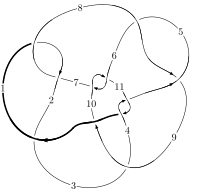
\includegraphics[width=112pt]{../../../GIT/diagram.site/Diagrams/png/758_11n_142.png}\\
\ \ \ A knot diagram\footnotemark}&
\allowdisplaybreaks
\textbf{Linearized knot diagam} \\
\cline{2-2}
 &
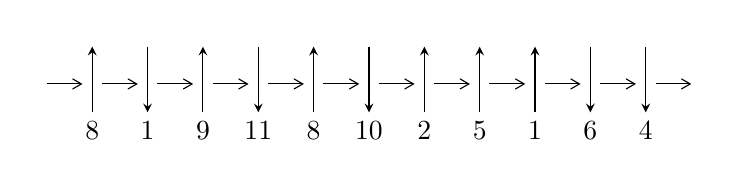
\begin{tikzpicture}[x=20pt, y=17pt]
	% nodes
	\node (C0) at (0, 0) {};
	\node (C1) at (1, 0) {};
	\node (C1U) at (1, +1) {};
	\node (C1D) at (1, -1) {8};

	\node (C2) at (2, 0) {};
	\node (C2U) at (2, +1) {};
	\node (C2D) at (2, -1) {1};

	\node (C3) at (3, 0) {};
	\node (C3U) at (3, +1) {};
	\node (C3D) at (3, -1) {9};

	\node (C4) at (4, 0) {};
	\node (C4U) at (4, +1) {};
	\node (C4D) at (4, -1) {11};

	\node (C5) at (5, 0) {};
	\node (C5U) at (5, +1) {};
	\node (C5D) at (5, -1) {8};

	\node (C6) at (6, 0) {};
	\node (C6U) at (6, +1) {};
	\node (C6D) at (6, -1) {10};

	\node (C7) at (7, 0) {};
	\node (C7U) at (7, +1) {};
	\node (C7D) at (7, -1) {2};

	\node (C8) at (8, 0) {};
	\node (C8U) at (8, +1) {};
	\node (C8D) at (8, -1) {5};

	\node (C9) at (9, 0) {};
	\node (C9U) at (9, +1) {};
	\node (C9D) at (9, -1) {1};

	\node (C10) at (10, 0) {};
	\node (C10U) at (10, +1) {};
	\node (C10D) at (10, -1) {6};

	\node (C11) at (11, 0) {};
	\node (C11U) at (11, +1) {};
	\node (C11D) at (11, -1) {4};
	\node (C12) at (12, 0) {};

	% arrows
	\draw[->,>={angle 60}]
	(C0) edge (C1) (C1) edge (C2) (C2) edge (C3) (C3) edge (C4) (C4) edge (C5) (C5) edge (C6) (C6) edge (C7) (C7) edge (C8) (C8) edge (C9) (C9) edge (C10) (C10) edge (C11) (C11) edge (C12) ;	\draw[->,>=stealth]
	(C1D) edge (C1U) (C2U) edge (C2D) (C3D) edge (C3U) (C4U) edge (C4D) (C5D) edge (C5U) (C6U) edge (C6D) (C7D) edge (C7U) (C8D) edge (C8U) (C9D) edge (C9U) (C10U) edge (C10D) (C11U) edge (C11D) ;
	\end{tikzpicture} \\
\hhline{~~} \\& 
\textbf{Solving Sequence} \\ \cline{2-2} 
 &
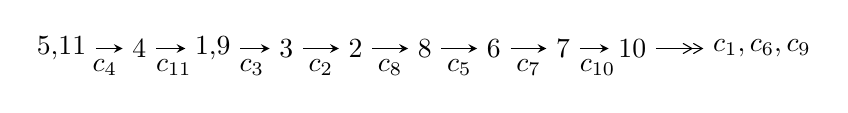
\begin{tikzpicture}[x=25pt, y=7pt]
	% node
	\node (A0) at (-1/8, 0) {5,11};
	\node (A1) at (1, 0) {4};
	\node (A2) at (33/16, 0) {1,9};
	\node (A3) at (25/8, 0) {3};
	\node (A4) at (33/8, 0) {2};
	\node (A5) at (41/8, 0) {8};
	\node (A6) at (49/8, 0) {6};
	\node (A7) at (57/8, 0) {7};
	\node (A8) at (65/8, 0) {10};
	\node (C1) at (1/2, -1) {$c_{4}$};
	\node (C2) at (3/2, -1) {$c_{11}$};
	\node (C3) at (21/8, -1) {$c_{3}$};
	\node (C4) at (29/8, -1) {$c_{2}$};
	\node (C5) at (37/8, -1) {$c_{8}$};
	\node (C6) at (45/8, -1) {$c_{5}$};
	\node (C7) at (53/8, -1) {$c_{7}$};
	\node (C8) at (61/8, -1) {$c_{10}$};
	\node (A9) at (10, 0) {$c_{1},c_{6},c_{9}$};

	% edge
	\draw[->,>=stealth]	
	(A0) edge (A1) (A1) edge (A2) (A2) edge (A3) (A3) edge (A4) (A4) edge (A5) (A5) edge (A6) (A6) edge (A7) (A7) edge (A8) ;
	\draw[->>,>={angle 60}]	
	(A8) edge (A9);
\end{tikzpicture} \\ 

\end{tabular} \\

\footnotetext{
The image of knot diagram is generated by the software ``\textbf{Draw programme}" developed by Andrew Bartholomew(\url{http://www.layer8.co.uk/maths/draw/index.htm\#Running-draw}), where we modified some parts for our purpose(\url{https://github.com/CATsTAILs/LinksPainter}).
}\phantom \\ \newline 
\centering \textbf{Ideals for irreducible components\footnotemark of $X_{\text{par}}$} 
 
\begin{align*}
I^u_{1}&=\langle 
- u^{13}+6 u^{12}+\cdots+b+3,\\
\phantom{I^u_{1}}&\phantom{= \langle  }u^{13}- u^{12}+15 u^{10}-48 u^9+106 u^8-178 u^7+222 u^6-230 u^5+175 u^4-107 u^3+57 u^2+2 a-19 u+10,\\
\phantom{I^u_{1}}&\phantom{= \langle  }u^{14}-5 u^{13}+\cdots-6 u+2\rangle \\
I^u_{2}&=\langle 
u^6+u^5+4 u^4+3 u^3+4 u^2+b+2 u+1,\;- u^7-2 u^5+2 u^4+3 u^3+4 u^2+2 a+4 u+1,\\
\phantom{I^u_{2}}&\phantom{= \langle  }u^8+2 u^7+6 u^6+8 u^5+11 u^4+10 u^3+8 u^2+5 u+2\rangle \\
I^u_{3}&=\langle 
u^4 a+2 u^2 a- u^3- a u+b+a- u+1,\;u^3 a+2 u^4+2 u^2 a+3 u^3+a^2+2 a u+5 u^2+2 a+u-1,\\
\phantom{I^u_{3}}&\phantom{= \langle  }u^5+u^4+2 u^3+u^2+u+1\rangle \\
\\
\end{align*}
\raggedright * 3 irreducible components of $\dim_{\mathbb{C}}=0$, with total 32 representations.\\
\footnotetext{All coefficients of polynomials are rational numbers. But the coefficients are sometimes approximated in decimal forms when there is not enough margin.}
\newpage
\renewcommand{\arraystretch}{1}
\centering \section*{I. $I^u_{1}= \langle - u^{13}+6 u^{12}+\cdots+b+3,\;u^{13}- u^{12}+\cdots+2 a+10,\;u^{14}-5 u^{13}+\cdots-6 u+2 \rangle$}
\flushleft \textbf{(i) Arc colorings}\\
\begin{tabular}{m{7pt} m{180pt} m{7pt} m{180pt} }
\flushright $a_{5}=$&$\begin{pmatrix}1\\0\end{pmatrix}$ \\
\flushright $a_{11}=$&$\begin{pmatrix}0\\u\end{pmatrix}$ \\
\flushright $a_{4}=$&$\begin{pmatrix}1\\- u^2\end{pmatrix}$ \\
\flushright $a_{1}=$&$\begin{pmatrix}- u\\u^3+u\end{pmatrix}$ \\
\flushright $a_{9}=$&$\begin{pmatrix}-\frac{1}{2} u^{13}+\frac{1}{2} u^{12}+\cdots+\frac{19}{2} u-5\\u^{13}-6 u^{12}+\cdots+11 u-3\end{pmatrix}$ \\
\flushright $a_{3}=$&$\begin{pmatrix}\frac{1}{2} u^{13}-\frac{5}{2} u^{12}+\cdots-\frac{11}{2} u^2+\frac{3}{2} u\\u^{13}-4 u^{12}+\cdots+3 u-1\end{pmatrix}$ \\
\flushright $a_{2}=$&$\begin{pmatrix}\frac{1}{2} u^{13}-\frac{3}{2} u^{12}+\cdots-\frac{7}{2} u^2+\frac{1}{2} u\\- u^{13}+4 u^{12}+\cdots-2 u+1\end{pmatrix}$ \\
\flushright $a_{8}=$&$\begin{pmatrix}-\frac{3}{2} u^{13}+\frac{13}{2} u^{12}+\cdots-\frac{3}{2} u-2\\u^{13}-6 u^{12}+\cdots+11 u-3\end{pmatrix}$ \\
\flushright $a_{6}=$&$\begin{pmatrix}\frac{3}{2} u^{13}-\frac{13}{2} u^{12}+\cdots-\frac{31}{2} u^2+\frac{13}{2} u\\- u^{13}+5 u^{12}+\cdots-8 u+3\end{pmatrix}$ \\
\flushright $a_{7}=$&$\begin{pmatrix}-2 u^{13}+9 u^{12}+\cdots+19 u^2-6 u\\u^{13}-4 u^{12}+\cdots+11 u-4\end{pmatrix}$ \\
\flushright $a_{10}=$&$\begin{pmatrix}-\frac{3}{2} u^{13}+\frac{13}{2} u^{12}+\cdots-\frac{3}{2} u-1\\u^{13}-5 u^{12}+\cdots+14 u-5\end{pmatrix}$\\ \flushright $a_{10}=$&$\begin{pmatrix}-\frac{3}{2} u^{13}+\frac{13}{2} u^{12}+\cdots-\frac{3}{2} u-1\\u^{13}-5 u^{12}+\cdots+14 u-5\end{pmatrix}$\\&\end{tabular}
\flushleft \textbf{(ii) Obstruction class $= -1$}\\~\\
\flushleft \textbf{(iii) Cusp Shapes $= -2 u^{13}+11 u^{12}-40 u^{11}+102 u^{10}-203 u^9+326 u^8-425 u^7+456 u^6-399 u^5+283 u^4-172 u^3+85 u^2-36 u+14$}\\~\\
\newpage\renewcommand{\arraystretch}{1}
\flushleft \textbf{(iv) u-Polynomials at the component}\newline \\
\begin{tabular}{m{50pt}|m{274pt}}
Crossings & \hspace{64pt}u-Polynomials at each crossing \\
\hline $$\begin{aligned}c_{1},c_{3},c_{7}\end{aligned}$$&$\begin{aligned}
&u^{14}+11 u^{12}+\cdots- u+1
\end{aligned}$\\
\hline $$\begin{aligned}c_{2}\end{aligned}$$&$\begin{aligned}
&u^{14}+22 u^{13}+\cdots+u+1
\end{aligned}$\\
\hline $$\begin{aligned}c_{4},c_{11}\end{aligned}$$&$\begin{aligned}
&u^{14}-5 u^{13}+\cdots-6 u+2
\end{aligned}$\\
\hline $$\begin{aligned}c_{5},c_{8}\end{aligned}$$&$\begin{aligned}
&u^{14}+8 u^{12}+\cdots-4 u+1
\end{aligned}$\\
\hline $$\begin{aligned}c_{6},c_{10}\end{aligned}$$&$\begin{aligned}
&u^{14}+11 u^{13}+\cdots+208 u+32
\end{aligned}$\\
\hline $$\begin{aligned}c_{9}\end{aligned}$$&$\begin{aligned}
&u^{14}+u^{13}+\cdots-42 u+43
\end{aligned}$\\
\hline
\end{tabular}\\~\\
\newpage\renewcommand{\arraystretch}{1}
\flushleft \textbf{(v) Riley Polynomials at the component}\newline \\
\begin{tabular}{m{50pt}|m{274pt}}
Crossings & \hspace{64pt}Riley Polynomials at each crossing \\
\hline $$\begin{aligned}c_{1},c_{3},c_{7}\end{aligned}$$&$\begin{aligned}
&y^{14}+22 y^{13}+\cdots+y+1
\end{aligned}$\\
\hline $$\begin{aligned}c_{2}\end{aligned}$$&$\begin{aligned}
&y^{14}-66 y^{13}+\cdots+57 y+1
\end{aligned}$\\
\hline $$\begin{aligned}c_{4},c_{11}\end{aligned}$$&$\begin{aligned}
&y^{14}+11 y^{13}+\cdots+48 y+4
\end{aligned}$\\
\hline $$\begin{aligned}c_{5},c_{8}\end{aligned}$$&$\begin{aligned}
&y^{14}+16 y^{13}+\cdots+6 y+1
\end{aligned}$\\
\hline $$\begin{aligned}c_{6},c_{10}\end{aligned}$$&$\begin{aligned}
&y^{14}+5 y^{13}+\cdots+4352 y+1024
\end{aligned}$\\
\hline $$\begin{aligned}c_{9}\end{aligned}$$&$\begin{aligned}
&y^{14}+29 y^{13}+\cdots-6924 y+1849
\end{aligned}$\\
\hline
\end{tabular}\\~\\
\newpage\flushleft \textbf{(vi) Complex Volumes and Cusp Shapes}
$$\begin{array}{c|c|c}  
\text{Solutions to }I^u_{1}& \I (\text{vol} + \sqrt{-1}CS) & \text{Cusp shape}\\
 \hline 
\begin{aligned}
u &= \phantom{-}0.287050 + 0.917286 I \\
a &= \phantom{-}1.72431 - 0.08692 I \\
b &= \phantom{-}0.75441 - 1.21287 I\end{aligned}
 & \phantom{-}0.82198 - 3.62125 I & \phantom{-}2.13881 + 1.61924 I \\ \hline\begin{aligned}
u &= \phantom{-}0.287050 - 0.917286 I \\
a &= \phantom{-}1.72431 + 0.08692 I \\
b &= \phantom{-}0.75441 + 1.21287 I\end{aligned}
 & \phantom{-}0.82198 + 3.62125 I & \phantom{-}2.13881 - 1.61924 I \\ \hline\begin{aligned}
u &= \phantom{-}1.148320 + 0.063656 I \\
a &= \phantom{-}0.028321 - 0.233596 I \\
b &= -0.38125 - 1.63279 I\end{aligned}
 & -14.6114 + 5.0048 I & -3.11103 - 2.22395 I \\ \hline\begin{aligned}
u &= \phantom{-}1.148320 - 0.063656 I \\
a &= \phantom{-}0.028321 + 0.233596 I \\
b &= -0.38125 + 1.63279 I\end{aligned}
 & -14.6114 - 5.0048 I & -3.11103 + 2.22395 I \\ \hline\begin{aligned}
u &= \phantom{-}0.151463 + 0.669236 I \\
a &= -1.172520 + 0.541864 I \\
b &= -0.010117 + 0.820058 I\end{aligned}
 & \phantom{-}0.100921 + 1.074380 I & \phantom{-}3.38569 - 3.60575 I \\ \hline\begin{aligned}
u &= \phantom{-}0.151463 - 0.669236 I \\
a &= -1.172520 - 0.541864 I \\
b &= -0.010117 - 0.820058 I\end{aligned}
 & \phantom{-}0.100921 - 1.074380 I & \phantom{-}3.38569 + 3.60575 I \\ \hline\begin{aligned}
u &= -0.137919 + 0.533558 I \\
a &= -0.824651 + 0.595460 I \\
b &= -0.029422 + 0.445046 I\end{aligned}
 & \phantom{-}0.158278 + 1.072210 I & \phantom{-}2.34747 - 5.95960 I \\ \hline\begin{aligned}
u &= -0.137919 - 0.533558 I \\
a &= -0.824651 - 0.595460 I \\
b &= -0.029422 - 0.445046 I\end{aligned}
 & \phantom{-}0.158278 - 1.072210 I & \phantom{-}2.34747 + 5.95960 I \\ \hline\begin{aligned}
u &= -0.12127 + 1.46215 I \\
a &= \phantom{-}0.495610 + 0.295894 I \\
b &= \phantom{-}0.459360 - 0.015268 I\end{aligned}
 & \phantom{-}6.08599 + 2.02171 I & \phantom{-}9.26276 - 3.22644 I \\ \hline\begin{aligned}
u &= -0.12127 - 1.46215 I \\
a &= \phantom{-}0.495610 - 0.295894 I \\
b &= \phantom{-}0.459360 + 0.015268 I\end{aligned}
 & \phantom{-}6.08599 - 2.02171 I & \phantom{-}9.26276 + 3.22644 I\\
 \hline 
 \end{array}$$\newpage$$\begin{array}{c|c|c}  
\text{Solutions to }I^u_{1}& \I (\text{vol} + \sqrt{-1}CS) & \text{Cusp shape}\\
 \hline 
\begin{aligned}
u &= \phantom{-}0.60561 + 1.35177 I \\
a &= -1.56827 + 0.69249 I \\
b &= -0.78424 + 1.62391 I\end{aligned}
 & -10.6271 - 11.1808 I & -0.33111 + 5.29605 I \\ \hline\begin{aligned}
u &= \phantom{-}0.60561 - 1.35177 I \\
a &= -1.56827 - 0.69249 I \\
b &= -0.78424 - 1.62391 I\end{aligned}
 & -10.6271 + 11.1808 I & -0.33111 - 5.29605 I \\ \hline\begin{aligned}
u &= \phantom{-}0.56676 + 1.45000 I \\
a &= \phantom{-}0.817208 - 1.060380 I \\
b &= -0.008750 - 1.377190 I\end{aligned}
 & -9.89254 - 1.11324 I & -1.192579 + 0.716159 I \\ \hline\begin{aligned}
u &= \phantom{-}0.56676 - 1.45000 I \\
a &= \phantom{-}0.817208 + 1.060380 I \\
b &= -0.008750 + 1.377190 I\end{aligned}
 & -9.89254 + 1.11324 I & -1.192579 - 0.716159 I\\
 \hline 
 \end{array}$$\newpage\newpage\renewcommand{\arraystretch}{1}
\centering \section*{II. $I^u_{2}= \langle u^6+u^5+4 u^4+3 u^3+4 u^2+b+2 u+1,\;- u^7-2 u^5+2 u^4+3 u^3+4 u^2+2 a+4 u+1,\;u^8+2 u^7+\cdots+5 u+2 \rangle$}
\flushleft \textbf{(i) Arc colorings}\\
\begin{tabular}{m{7pt} m{180pt} m{7pt} m{180pt} }
\flushright $a_{5}=$&$\begin{pmatrix}1\\0\end{pmatrix}$ \\
\flushright $a_{11}=$&$\begin{pmatrix}0\\u\end{pmatrix}$ \\
\flushright $a_{4}=$&$\begin{pmatrix}1\\- u^2\end{pmatrix}$ \\
\flushright $a_{1}=$&$\begin{pmatrix}- u\\u^3+u\end{pmatrix}$ \\
\flushright $a_{9}=$&$\begin{pmatrix}\frac{1}{2} u^7+u^5- u^4-\frac{3}{2} u^3-2 u^2-2 u-\frac{1}{2}\\- u^6- u^5-4 u^4-3 u^3-4 u^2-2 u-1\end{pmatrix}$ \\
\flushright $a_{3}=$&$\begin{pmatrix}-\frac{1}{2} u^7-2 u^6+\cdots-2 u+\frac{1}{2}\\- u^7-2 u^6-5 u^5-6 u^4-6 u^3-5 u^2-2 u-1\end{pmatrix}$ \\
\flushright $a_{2}=$&$\begin{pmatrix}\frac{1}{2} u^7+u^5- u^4-\frac{1}{2} u^3- u^2- u+\frac{1}{2}\\- u^7-2 u^6-5 u^5-6 u^4-5 u^3-4 u^2- u-1\end{pmatrix}$ \\
\flushright $a_{8}=$&$\begin{pmatrix}\frac{1}{2} u^7+u^6+2 u^5+3 u^4+\frac{3}{2} u^3+2 u^2+\frac{1}{2}\\- u^6- u^5-4 u^4-3 u^3-4 u^2-2 u-1\end{pmatrix}$ \\
\flushright $a_{6}=$&$\begin{pmatrix}-\frac{1}{2} u^7- u^6+\cdots-2 u-\frac{1}{2}\\u^5+u^4+3 u^3+2 u^2+u+1\end{pmatrix}$ \\
\flushright $a_{7}=$&$\begin{pmatrix}u^2+u+1\\u^6+2 u^5+4 u^4+5 u^3+4 u^2+2 u\end{pmatrix}$ \\
\flushright $a_{10}=$&$\begin{pmatrix}\frac{1}{2} u^7+u^6+\cdots+2 u+\frac{3}{2}\\- u^6- u^5-4 u^4-3 u^3-4 u^2- u-1\end{pmatrix}$\\ \flushright $a_{10}=$&$\begin{pmatrix}\frac{1}{2} u^7+u^6+\cdots+2 u+\frac{3}{2}\\- u^6- u^5-4 u^4-3 u^3-4 u^2- u-1\end{pmatrix}$\\&\end{tabular}
\flushleft \textbf{(ii) Obstruction class $= 1$}\\~\\
\flushleft \textbf{(iii) Cusp Shapes $= -3 u^7-6 u^6-15 u^5-22 u^4-22 u^3-22 u^2-13 u-6$}\\~\\
\newpage\renewcommand{\arraystretch}{1}
\flushleft \textbf{(iv) u-Polynomials at the component}\newline \\
\begin{tabular}{m{50pt}|m{274pt}}
Crossings & \hspace{64pt}u-Polynomials at each crossing \\
\hline $$\begin{aligned}c_{1}\end{aligned}$$&$\begin{aligned}
&u^8+4 u^6+u^5+4 u^4+3 u^3+3 u^2+u+1
\end{aligned}$\\
\hline $$\begin{aligned}c_{2}\end{aligned}$$&$\begin{aligned}
&u^8+8 u^7+24 u^6+37 u^5+36 u^4+21 u^3+11 u^2+5 u+1
\end{aligned}$\\
\hline $$\begin{aligned}c_{3},c_{7}\end{aligned}$$&$\begin{aligned}
&u^8+4 u^6- u^5+4 u^4-3 u^3+3 u^2- u+1
\end{aligned}$\\
\hline $$\begin{aligned}c_{4}\end{aligned}$$&$\begin{aligned}
&u^8+2 u^7+6 u^6+8 u^5+11 u^4+10 u^3+8 u^2+5 u+2
\end{aligned}$\\
\hline $$\begin{aligned}c_{5}\end{aligned}$$&$\begin{aligned}
&u^8+u^6-3 u^5+u^4-2 u^3+3 u^2+1
\end{aligned}$\\
\hline $$\begin{aligned}c_{6}\end{aligned}$$&$\begin{aligned}
&u^8+3 u^6+2 u^5+u^4+3 u^3+u^2+1
\end{aligned}$\\
\hline $$\begin{aligned}c_{8}\end{aligned}$$&$\begin{aligned}
&u^8+u^6+3 u^5+u^4+2 u^3+3 u^2+1
\end{aligned}$\\
\hline $$\begin{aligned}c_{9}\end{aligned}$$&$\begin{aligned}
&u^8+u^7+4 u^6+u^4-2 u^2+1
\end{aligned}$\\
\hline $$\begin{aligned}c_{10}\end{aligned}$$&$\begin{aligned}
&u^8+3 u^6-2 u^5+u^4-3 u^3+u^2+1
\end{aligned}$\\
\hline $$\begin{aligned}c_{11}\end{aligned}$$&$\begin{aligned}
&u^8-2 u^7+6 u^6-8 u^5+11 u^4-10 u^3+8 u^2-5 u+2
\end{aligned}$\\
\hline
\end{tabular}\\~\\
\newpage\renewcommand{\arraystretch}{1}
\flushleft \textbf{(v) Riley Polynomials at the component}\newline \\
\begin{tabular}{m{50pt}|m{274pt}}
Crossings & \hspace{64pt}Riley Polynomials at each crossing \\
\hline $$\begin{aligned}c_{1},c_{3},c_{7}\end{aligned}$$&$\begin{aligned}
&y^8+8 y^7+24 y^6+37 y^5+36 y^4+21 y^3+11 y^2+5 y+1
\end{aligned}$\\
\hline $$\begin{aligned}c_{2}\end{aligned}$$&$\begin{aligned}
&y^8-16 y^7+56 y^6+45 y^5+192 y^4+29 y^3-17 y^2-3 y+1
\end{aligned}$\\
\hline $$\begin{aligned}c_{4},c_{11}\end{aligned}$$&$\begin{aligned}
&y^8+8 y^7+26 y^6+44 y^5+41 y^4+20 y^3+8 y^2+7 y+4
\end{aligned}$\\
\hline $$\begin{aligned}c_{5},c_{8}\end{aligned}$$&$\begin{aligned}
&y^8+2 y^7+3 y^6- y^5-3 y^4+4 y^3+11 y^2+6 y+1
\end{aligned}$\\
\hline $$\begin{aligned}c_{6},c_{10}\end{aligned}$$&$\begin{aligned}
&y^8+6 y^7+11 y^6+4 y^5-3 y^4- y^3+3 y^2+2 y+1
\end{aligned}$\\
\hline $$\begin{aligned}c_{9}\end{aligned}$$&$\begin{aligned}
&y^8+7 y^7+18 y^6+4 y^5-13 y^4+4 y^3+6 y^2-4 y+1
\end{aligned}$\\
\hline
\end{tabular}\\~\\
\newpage\flushleft \textbf{(vi) Complex Volumes and Cusp Shapes}
$$\begin{array}{c|c|c}  
\text{Solutions to }I^u_{2}& \I (\text{vol} + \sqrt{-1}CS) & \text{Cusp shape}\\
 \hline 
\begin{aligned}
u &= \phantom{-}0.255307 + 0.956150 I \\
a &= \phantom{-}1.69644 - 0.66169 I \\
b &= \phantom{-}1.095290 + 0.323314 I\end{aligned}
 & -5.22098 - 1.00599 I & \phantom{-}2.77337 + 0.09808 I \\ \hline\begin{aligned}
u &= \phantom{-}0.255307 - 0.956150 I \\
a &= \phantom{-}1.69644 + 0.66169 I \\
b &= \phantom{-}1.095290 - 0.323314 I\end{aligned}
 & -5.22098 + 1.00599 I & \phantom{-}2.77337 - 0.09808 I \\ \hline\begin{aligned}
u &= -0.420429 + 1.128350 I \\
a &= -1.43682 - 0.24968 I \\
b &= -0.744211 - 1.167310 I\end{aligned}
 & \phantom{-}1.09366 + 5.02764 I & \phantom{-}3.89133 - 6.50935 I \\ \hline\begin{aligned}
u &= -0.420429 - 1.128350 I \\
a &= -1.43682 + 0.24968 I \\
b &= -0.744211 + 1.167310 I\end{aligned}
 & \phantom{-}1.09366 - 5.02764 I & \phantom{-}3.89133 + 6.50935 I \\ \hline\begin{aligned}
u &= -0.669415 + 0.364330 I \\
a &= \phantom{-}0.671643 + 0.022513 I \\
b &= -0.279662 + 1.002820 I\end{aligned}
 & -1.22874 - 0.94773 I & -2.78542 + 1.04891 I \\ \hline\begin{aligned}
u &= -0.669415 - 0.364330 I \\
a &= \phantom{-}0.671643 - 0.022513 I \\
b &= -0.279662 - 1.002820 I\end{aligned}
 & -1.22874 + 0.94773 I & -2.78542 - 1.04891 I \\ \hline\begin{aligned}
u &= -0.16546 + 1.54832 I \\
a &= \phantom{-}0.318738 + 0.607785 I \\
b &= -0.071417 + 0.603353 I\end{aligned}
 & \phantom{-}5.35605 + 1.96927 I & -2.37928 - 1.80892 I \\ \hline\begin{aligned}
u &= -0.16546 - 1.54832 I \\
a &= \phantom{-}0.318738 - 0.607785 I \\
b &= -0.071417 - 0.603353 I\end{aligned}
 & \phantom{-}5.35605 - 1.96927 I & -2.37928 + 1.80892 I\\
 \hline 
 \end{array}$$\newpage\newpage\renewcommand{\arraystretch}{1}
\centering \section*{III. $I^u_{3}= \langle u^4 a+2 u^2 a- u^3- a u+b+a- u+1,\;u^3 a+2 u^4+\cdots+2 a-1,\;u^5+u^4+2 u^3+u^2+u+1 \rangle$}
\flushleft \textbf{(i) Arc colorings}\\
\begin{tabular}{m{7pt} m{180pt} m{7pt} m{180pt} }
\flushright $a_{5}=$&$\begin{pmatrix}1\\0\end{pmatrix}$ \\
\flushright $a_{11}=$&$\begin{pmatrix}0\\u\end{pmatrix}$ \\
\flushright $a_{4}=$&$\begin{pmatrix}1\\- u^2\end{pmatrix}$ \\
\flushright $a_{1}=$&$\begin{pmatrix}- u\\u^3+u\end{pmatrix}$ \\
\flushright $a_{9}=$&$\begin{pmatrix}a\\- u^4 a-2 u^2 a+u^3+a u- a+u-1\end{pmatrix}$ \\
\flushright $a_{3}=$&$\begin{pmatrix}2 u^3+4 u^2+a+4 u+4\\u^4 a+u^2 a+u^3- a u+a+u+1\end{pmatrix}$ \\
\flushright $a_{2}=$&$\begin{pmatrix}u^4 a+u^4+2 u^2 a+u^3+4 u^2+2 a+u+3\\- u^4 a- u^3 a- u^4-2 u^2 a+2 u^3- a u- a+3 u\end{pmatrix}$ \\
\flushright $a_{8}=$&$\begin{pmatrix}u^4 a+2 u^2 a- u^3- a u+2 a- u+1\\- u^4 a-2 u^2 a+u^3+a u- a+u-1\end{pmatrix}$ \\
\flushright $a_{6}=$&$\begin{pmatrix}- u^4- u^3-2 u^2- u-1\\- u^4 a+u^4- u^2 a+2 u^3+a u+2 u^2\end{pmatrix}$ \\
\flushright $a_{7}=$&$\begin{pmatrix}2 u^4+2 u^3+4 u^2+2 u+2\\2 u^4 a-2 u^4+2 u^2 a-4 u^3-2 a u-4 u^2- u\end{pmatrix}$ \\
\flushright $a_{10}=$&$\begin{pmatrix}- u^4- u^3-2 u^2- u-1\\- u^4 a+u^4- u^2 a+2 u^3+a u+2 u^2+u\end{pmatrix}$\\ \flushright $a_{10}=$&$\begin{pmatrix}- u^4- u^3-2 u^2- u-1\\- u^4 a+u^4- u^2 a+2 u^3+a u+2 u^2+u\end{pmatrix}$\\&\end{tabular}
\flushleft \textbf{(ii) Obstruction class $= -1$}\\~\\
\flushleft \textbf{(iii) Cusp Shapes $= 4 u^3+4 u^2+4 u-2$}\\~\\
\newpage\renewcommand{\arraystretch}{1}
\flushleft \textbf{(iv) u-Polynomials at the component}\newline \\
\begin{tabular}{m{50pt}|m{274pt}}
Crossings & \hspace{64pt}u-Polynomials at each crossing \\
\hline $$\begin{aligned}c_{1},c_{3},c_{7}\end{aligned}$$&$\begin{aligned}
&u^{10}- u^9+\cdots-20 u+23
\end{aligned}$\\
\hline $$\begin{aligned}c_{2}\end{aligned}$$&$\begin{aligned}
&u^{10}+15 u^9+\cdots+2268 u+529
\end{aligned}$\\
\hline $$\begin{aligned}c_{4},c_{11}\end{aligned}$$&$\begin{aligned}
&(u^5+u^4+2 u^3+u^2+u+1)^2
\end{aligned}$\\
\hline $$\begin{aligned}c_{5},c_{8}\end{aligned}$$&$\begin{aligned}
&u^{10}+5 u^9+\cdots+20 u+7
\end{aligned}$\\
\hline $$\begin{aligned}c_{6},c_{10}\end{aligned}$$&$\begin{aligned}
&(u-1)^{10}
\end{aligned}$\\
\hline $$\begin{aligned}c_{9}\end{aligned}$$&$\begin{aligned}
&u^{10}+u^9+10 u^8-8 u^7+42 u^6+2 u^5+29 u^4+43 u^3+28 u^2-12 u+67
\end{aligned}$\\
\hline
\end{tabular}\\~\\
\newpage\renewcommand{\arraystretch}{1}
\flushleft \textbf{(v) Riley Polynomials at the component}\newline \\
\begin{tabular}{m{50pt}|m{274pt}}
Crossings & \hspace{64pt}Riley Polynomials at each crossing \\
\hline $$\begin{aligned}c_{1},c_{3},c_{7}\end{aligned}$$&$\begin{aligned}
&y^{10}+15 y^9+\cdots+2268 y+529
\end{aligned}$\\
\hline $$\begin{aligned}c_{2}\end{aligned}$$&$\begin{aligned}
&y^{10}-33 y^9+\cdots-245284 y+279841
\end{aligned}$\\
\hline $$\begin{aligned}c_{4},c_{11}\end{aligned}$$&$\begin{aligned}
&(y^5+3 y^4+4 y^3+y^2- y-1)^2
\end{aligned}$\\
\hline $$\begin{aligned}c_{5},c_{8}\end{aligned}$$&$\begin{aligned}
&y^{10}+3 y^9+\cdots+468 y+49
\end{aligned}$\\
\hline $$\begin{aligned}c_{6},c_{10}\end{aligned}$$&$\begin{aligned}
&(y-1)^{10}
\end{aligned}$\\
\hline $$\begin{aligned}c_{9}\end{aligned}$$&$\begin{aligned}
&y^{10}+19 y^9+\cdots+3608 y+4489
\end{aligned}$\\
\hline
\end{tabular}\\~\\
\newpage\flushleft \textbf{(vi) Complex Volumes and Cusp Shapes}
$$\begin{array}{c|c|c}  
\text{Solutions to }I^u_{3}& \I (\text{vol} + \sqrt{-1}CS) & \text{Cusp shape}\\
 \hline 
\begin{aligned}
u &= \phantom{-}0.339110 + 0.822375 I \\
a &= \phantom{-}1.56543 - 1.34638 I \\
b &= -0.144990 + 0.454920 I\end{aligned}
 & -6.25064 - 1.53058 I & -5.48489 + 4.43065 I \\ \hline\begin{aligned}
u &= \phantom{-}0.339110 + 0.822375 I \\
a &= -2.47201 - 1.14141 I \\
b &= -2.06136 - 0.79577 I\end{aligned}
 & -6.25064 - 1.53058 I & -5.48489 + 4.43065 I \\ \hline\begin{aligned}
u &= \phantom{-}0.339110 - 0.822375 I \\
a &= \phantom{-}1.56543 + 1.34638 I \\
b &= -0.144990 - 0.454920 I\end{aligned}
 & -6.25064 + 1.53058 I & -5.48489 - 4.43065 I \\ \hline\begin{aligned}
u &= \phantom{-}0.339110 - 0.822375 I \\
a &= -2.47201 + 1.14141 I \\
b &= -2.06136 + 0.79577 I\end{aligned}
 & -6.25064 + 1.53058 I & -5.48489 - 4.43065 I \\ \hline\begin{aligned}
u &= -0.766826\phantom{ +0.000000I} \\
a &= -0.595741 + 0.396465 I \\
b &= -0.258559 - 1.303830 I\end{aligned}
 & -4.17865\phantom{ +0.000000I} & -4.51890\phantom{ +0.000000I} \\ \hline\begin{aligned}
u &= -0.766826\phantom{ +0.000000I} \\
a &= -0.595741 - 0.396465 I \\
b &= -0.258559 + 1.303830 I\end{aligned}
 & -4.17865\phantom{ +0.000000I} & -4.51890\phantom{ +0.000000I} \\ \hline\begin{aligned}
u &= -0.455697 + 1.200150 I \\
a &= \phantom{-}1.04040 + 1.01526 I \\
b &= \phantom{-}0.43147 + 1.63522 I\end{aligned}
 & -0.70717 + 4.40083 I & -1.25569 - 3.49859 I \\ \hline\begin{aligned}
u &= -0.455697 + 1.200150 I \\
a &= -1.53808 - 0.24695 I \\
b &= -0.466561 - 1.013320 I\end{aligned}
 & -0.70717 + 4.40083 I & -1.25569 - 3.49859 I \\ \hline\begin{aligned}
u &= -0.455697 - 1.200150 I \\
a &= \phantom{-}1.04040 - 1.01526 I \\
b &= \phantom{-}0.43147 - 1.63522 I\end{aligned}
 & -0.70717 - 4.40083 I & -1.25569 + 3.49859 I \\ \hline\begin{aligned}
u &= -0.455697 - 1.200150 I \\
a &= -1.53808 + 0.24695 I \\
b &= -0.466561 + 1.013320 I\end{aligned}
 & -0.70717 - 4.40083 I & -1.25569 + 3.49859 I\\
 \hline 
 \end{array}$$\newpage
\newpage\renewcommand{\arraystretch}{1}
\centering \section*{ IV. u-Polynomials}
\begin{tabular}{m{50pt}|m{274pt}}
Crossings & \hspace{64pt}u-Polynomials at each crossing \\
\hline $$\begin{aligned}c_{1}\end{aligned}$$&$\begin{aligned}
&(u^8+4 u^6+\cdots+u+1)(u^{10}- u^9+\cdots-20 u+23)\\
&\cdot(u^{14}+11 u^{12}+\cdots- u+1)
\end{aligned}$\\
\hline $$\begin{aligned}c_{2}\end{aligned}$$&$\begin{aligned}
&(u^8+8 u^7+24 u^6+37 u^5+36 u^4+21 u^3+11 u^2+5 u+1)\\
&\cdot(u^{10}+15 u^9+\cdots+2268 u+529)(u^{14}+22 u^{13}+\cdots+u+1)
\end{aligned}$\\
\hline $$\begin{aligned}c_{3},c_{7}\end{aligned}$$&$\begin{aligned}
&(u^8+4 u^6+\cdots- u+1)(u^{10}- u^9+\cdots-20 u+23)\\
&\cdot(u^{14}+11 u^{12}+\cdots- u+1)
\end{aligned}$\\
\hline $$\begin{aligned}c_{4}\end{aligned}$$&$\begin{aligned}
&(u^5+u^4+2 u^3+u^2+u+1)^2\\
&\cdot(u^8+2 u^7+6 u^6+8 u^5+11 u^4+10 u^3+8 u^2+5 u+2)\\
&\cdot(u^{14}-5 u^{13}+\cdots-6 u+2)
\end{aligned}$\\
\hline $$\begin{aligned}c_{5}\end{aligned}$$&$\begin{aligned}
&(u^8+u^6-3 u^5+u^4-2 u^3+3 u^2+1)(u^{10}+5 u^9+\cdots+20 u+7)\\
&\cdot(u^{14}+8 u^{12}+\cdots-4 u+1)
\end{aligned}$\\
\hline $$\begin{aligned}c_{6}\end{aligned}$$&$\begin{aligned}
&(u-1)^{10}(u^8+3 u^6+2 u^5+u^4+3 u^3+u^2+1)\\
&\cdot(u^{14}+11 u^{13}+\cdots+208 u+32)
\end{aligned}$\\
\hline $$\begin{aligned}c_{8}\end{aligned}$$&$\begin{aligned}
&(u^8+u^6+3 u^5+u^4+2 u^3+3 u^2+1)(u^{10}+5 u^9+\cdots+20 u+7)\\
&\cdot(u^{14}+8 u^{12}+\cdots-4 u+1)
\end{aligned}$\\
\hline $$\begin{aligned}c_{9}\end{aligned}$$&$\begin{aligned}
&(u^8+u^7+4 u^6+u^4-2 u^2+1)\\
&\cdot(u^{10}+u^9+10 u^8-8 u^7+42 u^6+2 u^5+29 u^4+43 u^3+28 u^2-12 u+67)\\
&\cdot(u^{14}+u^{13}+\cdots-42 u+43)
\end{aligned}$\\
\hline $$\begin{aligned}c_{10}\end{aligned}$$&$\begin{aligned}
&(u-1)^{10}(u^8+3 u^6-2 u^5+u^4-3 u^3+u^2+1)\\
&\cdot(u^{14}+11 u^{13}+\cdots+208 u+32)
\end{aligned}$\\
\hline $$\begin{aligned}c_{11}\end{aligned}$$&$\begin{aligned}
&(u^5+u^4+2 u^3+u^2+u+1)^2\\
&\cdot(u^8-2 u^7+6 u^6-8 u^5+11 u^4-10 u^3+8 u^2-5 u+2)\\
&\cdot(u^{14}-5 u^{13}+\cdots-6 u+2)
\end{aligned}$\\
\hline
\end{tabular}\newpage\renewcommand{\arraystretch}{1}
\centering \section*{ V. Riley Polynomials}
\begin{tabular}{m{50pt}|m{274pt}}
Crossings & \hspace{64pt}Riley Polynomials at each crossing \\
\hline $$\begin{aligned}c_{1},c_{3},c_{7}\end{aligned}$$&$\begin{aligned}
&(y^8+8 y^7+24 y^6+37 y^5+36 y^4+21 y^3+11 y^2+5 y+1)\\
&\cdot(y^{10}+15 y^9+\cdots+2268 y+529)(y^{14}+22 y^{13}+\cdots+y+1)
\end{aligned}$\\
\hline $$\begin{aligned}c_{2}\end{aligned}$$&$\begin{aligned}
&(y^8-16 y^7+56 y^6+45 y^5+192 y^4+29 y^3-17 y^2-3 y+1)\\
&\cdot(y^{10}-33 y^9+\cdots-245284 y+279841)(y^{14}-66 y^{13}+\cdots+57 y+1)
\end{aligned}$\\
\hline $$\begin{aligned}c_{4},c_{11}\end{aligned}$$&$\begin{aligned}
&(y^5+3 y^4+4 y^3+y^2- y-1)^2\\
&\cdot(y^8+8 y^7+26 y^6+44 y^5+41 y^4+20 y^3+8 y^2+7 y+4)\\
&\cdot(y^{14}+11 y^{13}+\cdots+48 y+4)
\end{aligned}$\\
\hline $$\begin{aligned}c_{5},c_{8}\end{aligned}$$&$\begin{aligned}
&(y^8+2 y^7+3 y^6- y^5-3 y^4+4 y^3+11 y^2+6 y+1)\\
&\cdot(y^{10}+3 y^9+\cdots+468 y+49)(y^{14}+16 y^{13}+\cdots+6 y+1)
\end{aligned}$\\
\hline $$\begin{aligned}c_{6},c_{10}\end{aligned}$$&$\begin{aligned}
&(y-1)^{10}(y^8+6 y^7+11 y^6+4 y^5-3 y^4- y^3+3 y^2+2 y+1)\\
&\cdot(y^{14}+5 y^{13}+\cdots+4352 y+1024)
\end{aligned}$\\
\hline $$\begin{aligned}c_{9}\end{aligned}$$&$\begin{aligned}
&(y^8+7 y^7+18 y^6+4 y^5-13 y^4+4 y^3+6 y^2-4 y+1)\\
&\cdot(y^{10}+19 y^9+\cdots+3608 y+4489)\\
&\cdot(y^{14}+29 y^{13}+\cdots-6924 y+1849)
\end{aligned}$\\
\hline
\end{tabular}
\vskip 2pc
\end{document}